\section{Static Friction}

The goal of this test is to determine the static friction over the whole range of motion. The static friction torque is the torque which is needed to move the end-effector from standstill. This test allows to make a statement about the transparency of the system without any compensation control implemented. 

\subsection{Implementation}

The range of motion is defined between $\pm$90° and it is driven in steps of 5°. The user has to define the current direction (positive is clockwise and negative is counter-clockwise). The profile is then also driven in this direction. The program runs full-automatic. In the end however, it does not stop automatically but has to be stopped manually. This can be done as soon as the last measurement is taken (the end-effector will go back to 0° and continue to do measurements for 0° forever). After a position setpoint is reached, the system starts to apply a current (by default in 0.001 A steps). Meanwhile, the position difference between two consecutive measurements is observed and as soon as the difference exceeds 0.015°, the current setpoint is saved as friction torque and is reset to zero. Afterwards, the system drives to a new position setpoint. Between the reaching of a position setpoint and the increasing of the current, the system waits a small amount of time and does nothing, since there could be some rest-movement, which would falsify the measurements of the friction torque.

\subsection{Data Analysis}

In order to analyse the results, the final current setpoints are recorded and assigend to the correct position. Since there can always be some measurement errors (mostly too low measurements), it is best to have multiple data sets. These different data sets can all be fed into the script at once. For each position, the largest friction torque measurement is taken. These measurements are then multiplied with the torque constant of the motor version in order to calculate the torque.

\subsection{Results}

In the following two plots, results for MIKE \#6 and MIKE \#3 can be seen. It is visible that the friction for MIKE \#6 seems to be slightly larger than for MIKE \#3. What is a little strange is that in the ICORR paper from 2019, the measurements are all higher. Maybe then the sealings of the bearings were not removed, increasing the friction a lot. The measurements presented here are all pretty consistent over the whole range of motion, there are a few outliers, which are probably due to small measurement errors.

\begin{figure}[h]
    \begin{minipage}[m]{0.48\textwidth}
     \centering
        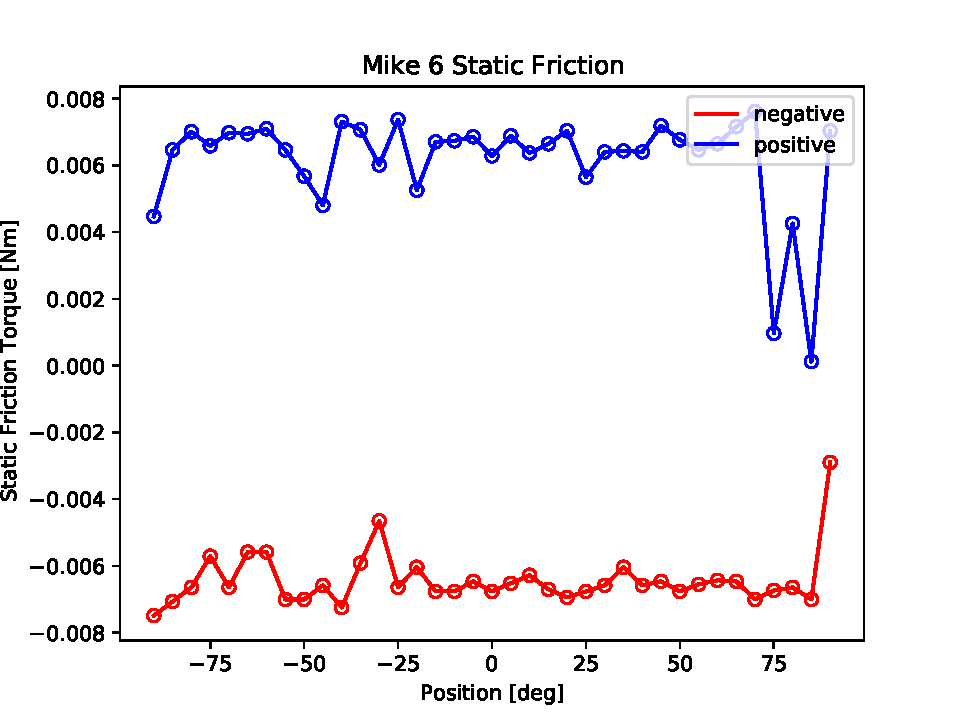
\includegraphics[width = \textwidth]{chapters/static friction/Mike6_StaticFriction.pdf}
    \end{minipage}
    \hfill
    \begin{minipage}[m]{0.48\textwidth}
     \centering
        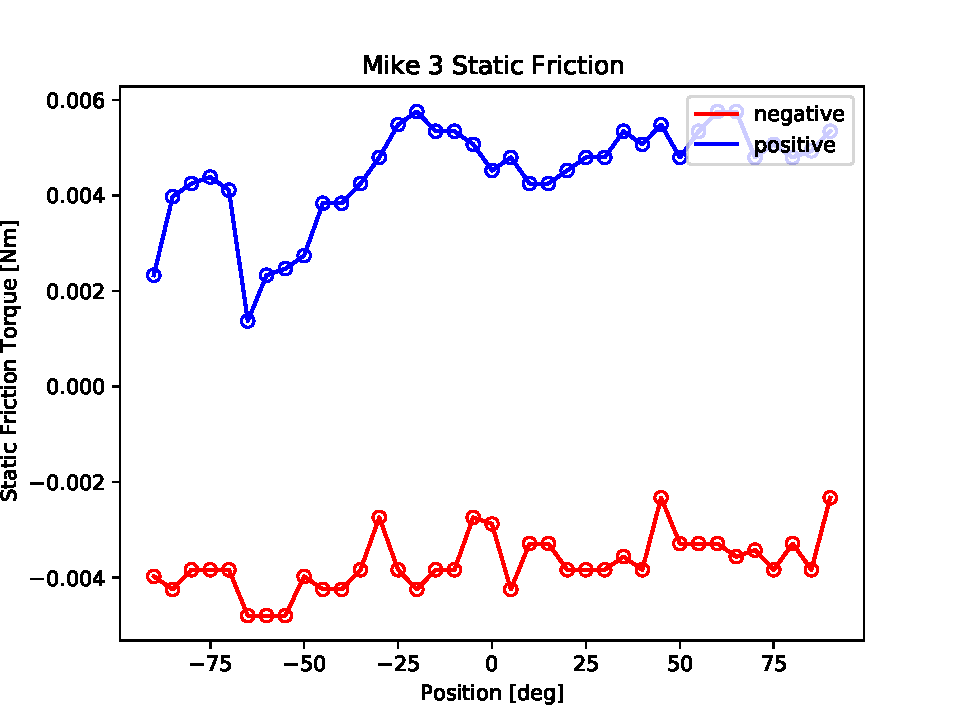
\includegraphics[width = \textwidth]{chapters/static friction/Mike3_StaticFriction.pdf}
    \end{minipage}
    \caption{Positive current equals clockwise and negative equals counter-clockwise; The profile was driven in the same direction as the current was applied, since this provides more friction. As can be seen, the static friction is low and therefore the system is very transparent without any control.}
\end{figure}

It is also important to mention that the current setpoint is used to evaluate the friction torque and not the estimated current. The next plot shows the current setpoint and the measured current in a cutout from a static friction dataset: 

\begin{figure}[h]
    \begin{minipage}[m]{0.48\textwidth}
     \centering
        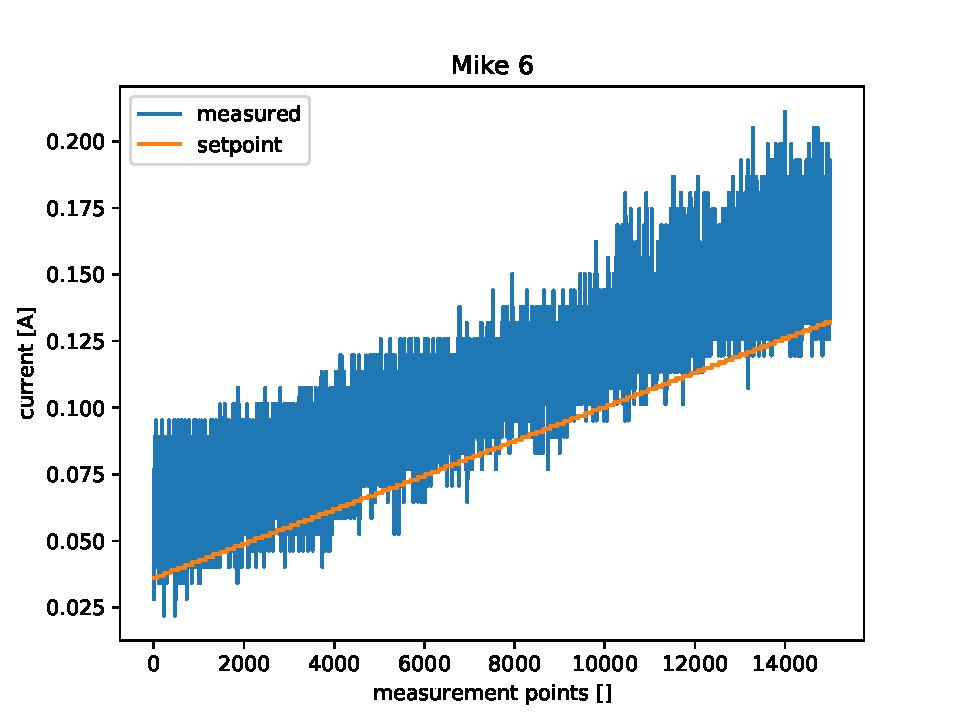
\includegraphics[width = \textwidth]{chapters/static friction/current.pdf}
    \end{minipage}
    \hfill
    \begin{minipage}[m]{0.48\textwidth}
     \centering
        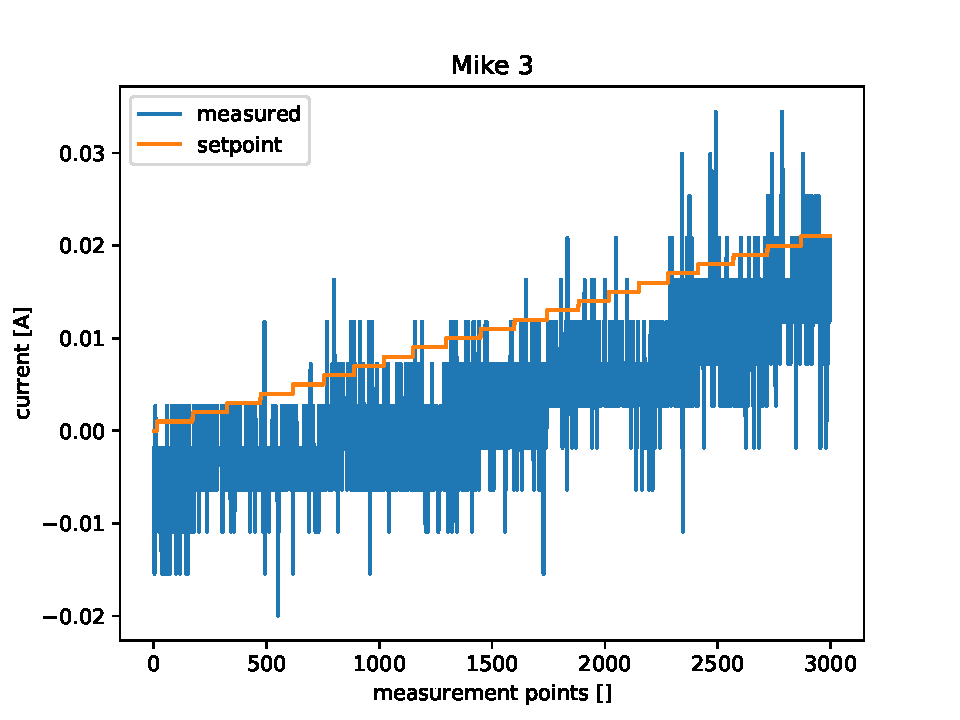
\includegraphics[width = \textwidth]{chapters/static friction/current_3.pdf}
    \end{minipage}
    \caption{The plot shows the measured as well as the desired current.}
\end{figure}

It is visible that the measured current is noisy and always seems to have an offset from the setpoint, which has to be taken into account when analysing the results. \\

Another observation was that there is a strong dependency on the direction in which the position profile is driven. In more detail, the friction torque is much higher when the profile is driven in the same direction as the current is applied. For example if a negative (counter-clockwise) current is applied, the friction torque is higher if the profile is driven counter-clockwise (90° to -90°) than when it is driven clockwise (-90° to 90°). This behaviour was observed for both devices MIKE \#6 and MIKE \#3 and is visualized in the following plot (recordings of MIKE \#3). This is why it is enough to run the profile only in the direction with more friction as described earlier.

\begin{figure}
    \centering
    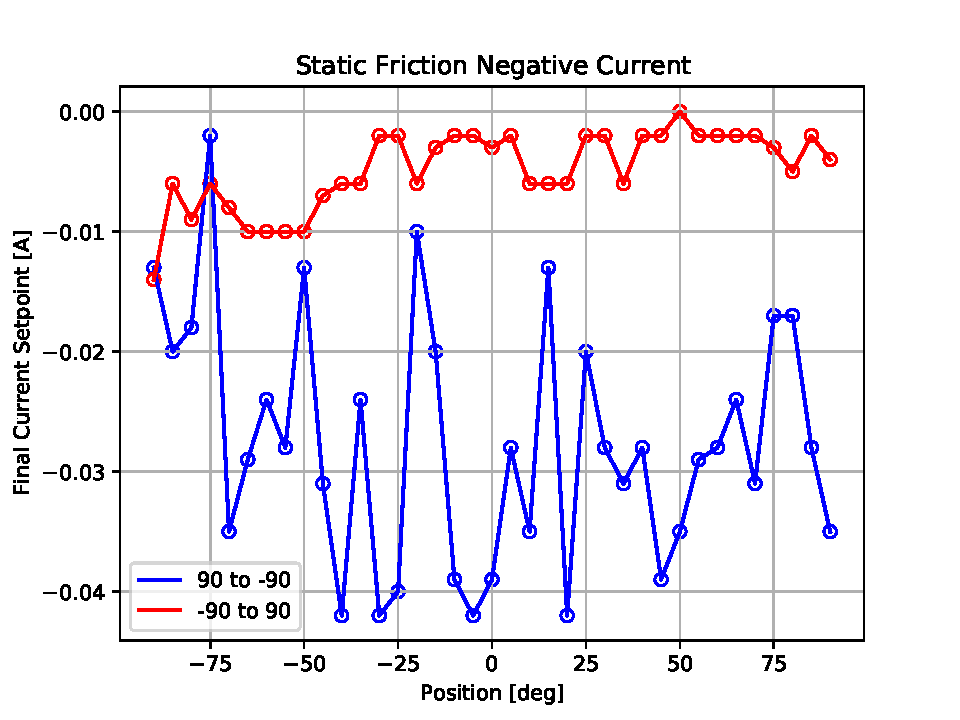
\includegraphics[width = 0.6\textwidth]{chapters/static friction/cw_vs_ccw.pdf}
    \caption{Here the direction dependency is visualized. The profile was driven in clockwise and counter-clockwise direction, while the applied current was negative (CCW) in both cases.}
\end{figure}